% $Header$

\documentclass{beamer}

% This file is a solution template for:

% - Talk at a conference/colloquium.
% - Talk length is about 20min.
% - Style is ornate.



% Copyright 2004 by Till Tantau <tantau@users.sourceforge.net>.
%
% In principle, this file can be redistributed and/or modified under
% the terms of the GNU Public License, version 2.
%
% However, this file is supposed to be a template to be modified
% for your own needs. For this reason, if you use this file as a
% template and not specifically distribute it as part of a another
% package/program, I grant the extra permission to freely copy and
% modify this file as you see fit and even to delete this copyright
% notice. 


%\mode<presentation>
%{
%  \usetheme{Warsaw}
%  % or ...
%
%  \setbeamercovered{transparent}
%  % or whatever (possibly just delete it)
%}
%
%
%\usepackage[english]{babel}
%% or whatever
%
%\usepackage[latin1]{inputenc}
%% or whatever
%
%\usepackage{times}
%\usepackage[T1]{fontenc}
%% Or whatever. Note that the encoding and the font should match. If T1
%% does not look nice, try deleting the line with the fontenc.




% Setup appearance:
\mode<presentation>
{
\usetheme{Darmstadt}
\usefonttheme[onlylarge]{structurebold}
\setbeamerfont*{frametitle}{size=\normalsize,series=\bfseries}
\setbeamertemplate{navigation symbols}{}
\usefonttheme{professionalfonts}
}

% Standard packages

\usepackage[english]{babel}
\usepackage[latin1]{inputenc}
\usepackage{times}
\usepackage[T1]{fontenc}

%
%\usefonttheme[onlymath]{serif}


% Setup TikZ

\usepackage{tikz}
\usetikzlibrary{arrows}
\tikzstyle{block}=[draw opacity=0.7,line width=1.4cm]




\title[AUV control without linear velocity measurements] % (optional, use only with long paper titles)
{Inertial-aided Homography-based Visual Servo Control of Autonomous Underwater Vehicles without Linear Velocity Measurements}

%\subtitle
%{Include Only If Paper Has a Subtitle}

%\author[Author, Another] % (optional, use only with lots of authors)
%{F.~Author\inst{1} \and S.~Another\inst{2}}
% - Give the names in the same order as the appear in the paper.
% - Use the \inst{?} command only if the authors have different
%   affiliation.

%\institute[Universities of Somewhere and Elsewhere] % (optional, but mostly needed)
%{
%  \inst{1}%
% Department of Computer Science\\
% University of Somewhere
% \and
%  \inst{2}%
%  Department of Theoretical Philosophy\\
%  University of Elsewhere}
% - Use the \inst command only if there are several affiliations.
% - Keep it simple, no one is interested in your street address.

\author[Nguyen, Hua, Allibert and Hamel] % (optional, use only with lots of authors)
{L.-H.~Nguyen \and M.-D.~Hua \and G.~Allibert \and T.~Hamel}
\institute[Universities of Somewhere and Elsewhere] % (optional, but mostly needed)
{
	\textit{Universit\'e C\^ote d'Azur, CNRS, I3S}\\
	Sophia Antipolis, France \\
	lhnguyen(hua,allibert,thamel)@i3s.unice.fr}
	
	
\date[ICSTCC 2017] % (optional, should be abbreviation of conference name)
{21st ICSTCC, 2017}
% - Either use conference name or its abbreviation.
% - Not really informative to the audience, more for people (including
%   yourself) who are reading the slides online

%\subject{Theoretical Computer Science}
% This is only inserted into the PDF information catalog. Can be left
% out. 



% If you have a file called "university-logo-filename.xxx", where xxx
% is a graphic format that can be processed by latex or pdflatex,
% resp., then you can add a logo as follows:

% \pgfdeclareimage[height=0.5cm]{university-logo}{university-logo-filename}
% \logo{\pgfuseimage{university-logo}}



% Delete this, if you do not want the table of contents to pop up at
% the beginning of each subsection:
\AtBeginSubsection[]
{
  \begin{frame}<beamer>{Outline}
    \tableofcontents[currentsection,currentsubsection]
  \end{frame}
}


% If you wish to uncover everything in a step-wise fashion, uncomment
% the following command: 

%\beamerdefaultoverlayspecification{<+->}


\begin{document}

\begin{frame}
  \titlepage
\end{frame}

\begin{frame}{Outline}
  \tableofcontents
  % You might wish to add the option [pausesections]
\end{frame}


% Structuring a talk is a difficult task and the following structure
% may not be suitable. Here are some rules that apply for this
% solution: 

% - Exactly two or three sections (other than the summary).
% - At *most* three subsections per section.
% - Talk about 30s to 2min per frame. So there should be between about
%   15 and 30 frames, all told.

% - A conference audience is likely to know very little of what you
%   are going to talk about. So *simplify*!
% - In a 20min talk, getting the main ideas across is hard
%   enough. Leave out details, even if it means being less precise than
%   you think necessary.
% - If you omit details that are vital to the proof/implementation,
%   just say so once. Everybody will be happy with that.

\section{Motivation}

%\subsection{The Basic Problem}

\begin{frame}{Why Visual Servo Control?}
  % - A title should summarize the slide in an understandable fashion
  %   for anyone how does not follow everything on the slide itself.
%	\begin{figure}[ht!]
	%\centering
%		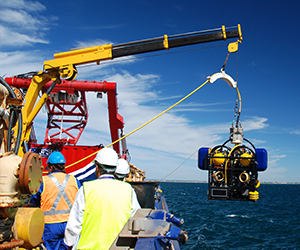
\includegraphics[width=30mm]{Images/ROV_operations_PRODUCT_IMAGE2.jpg}
%		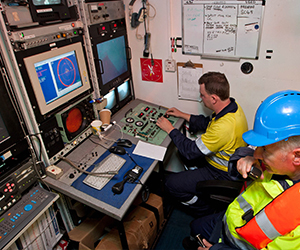
\includegraphics[width=30mm]{Images/ROV_operations_PRODUCT_IMAGE1.jpg}
%		\caption{ROV and its operation, source: www.jfdglobal.com}
%	\label{ROV}
%\end{figure}




	\begin{columns}[t]
		\column{.5\textwidth}	
		\begin{exampleblock}{Underwater issues:}		
			\begin{itemize}
				\item No GPS 
			\end{itemize}
		\end{exampleblock}
		\begin{exampleblock}{Camera}		
			\begin{itemize}
				\item Operation closed to structures
				\item Rich of informations
			\end{itemize}
		\end{exampleblock}
	
		
		\column{.5\textwidth}		
		\begin{exampleblock}{Stereo camera}
			\begin{itemize}
				\item Calculation power required
			\end{itemize}
		\end{exampleblock}
		\begin{exampleblock}{Monocular camera}
			\begin{itemize}
				\item More generic
			\end{itemize}
		\end{exampleblock}
	\end{columns}

\end{frame}

\begin{frame}{Linear velocity measurement}
	\begin{columns}[t]
		\column{.5\textwidth}
		\begin{exampleblock}{DVL issues:}
			\begin{itemize}
				\item High price
				\item High weight
				\item Violate maximum slope-threshold of DVLs in close proximity operation
			\end{itemize}
		\end{exampleblock}
		\column{.5\textwidth}
		
		
	\end{columns} 
\end{frame}

\begin{frame}{System modeling}
	\begin{columns}
		\column[content...]{.5\textwidth}
		\begin{figure}
			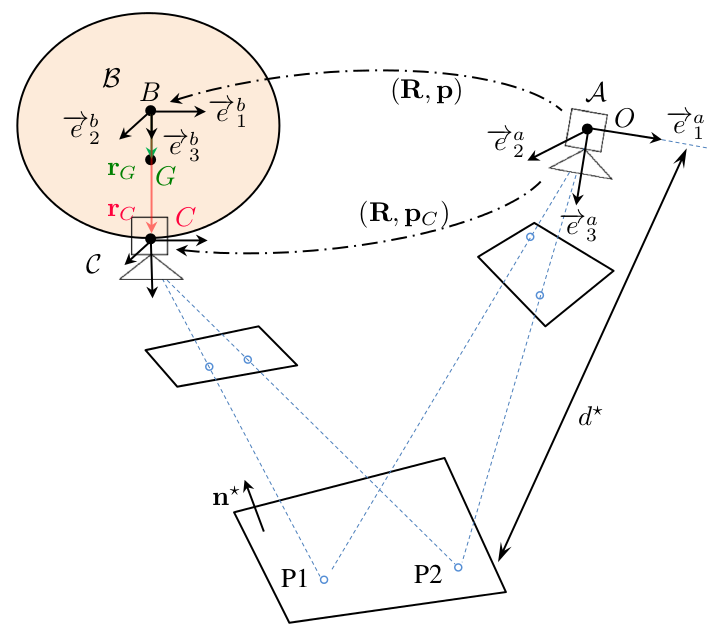
\includegraphics[width = 50mm]{Images/Notation.png}
		\end{figure}
		\column[placement]{.6\textwidth}
		\begin{block}{Equations of motion:}
			\scriptsize
			\begin{equation*}\label{eq:system2}
			\begin{array}{rl}
			\dot{\mathbf{p}} & =  \mathbf{R} \mathbf{V} \\
			\dot{\mathbf{R}} & =  \mathbf{R} \mathbf{\Omega}_\times \\
			\!\!\dot{\mathbf{P}}_h &= \mathbf{P}_h \times \mathbf{\Omega} +\mathbf{F}_c + \mathbf{F}_{gb} + \mathbf{F}_d  \\
			\!\!\dot{\mathbf{\Pi}}_h &=  \mathbf{\Pi}_h \!\times\! \mathbf{\mathbf{\Omega}} + \mathbf{P}_h \!\times \!\mathbf{V}_h  +\mathbf{\Gamma}_c + \mathbf{\Gamma}_g + \mathbf{\Gamma}_d \!\!\vspace{-0.2cm}
			\end{array}
			\end{equation*} \vspace{-0.3cm}
			where: \\
			\begin{equation*}
			\begin{array}{rl}
			\mathbf{P}_h & = \mathbf{M}\mathbf{V}_h + \mathbf{D}^{\!\top} \mathbf{\Omega}\\[1ex]
			\mathbf{\Pi}_h & = \mathbf{J} \mathbf{\Omega} + \mathbf{D}\mathbf{V}_h \\
			\mathbf{F}_{gb}  &\triangleq (m g - F_b) \mathbf{R}^{\!\top} \mathbf{e}_3\\
			\mathbf{\Gamma}_g  &\triangleq mgl\mathbf{e}_{3}\! \times \!\mathbf{R}^{\!\top} \mathbf{e}_3\\
			\mathbf{F}_d(\mathbf{V}_h) & = - (\mathbf{D}_{V\!l}   +|\mathbf{V}_h|\mathbf{D}_{V\!q} )\mathbf{V}_h  \\
			\mathbf{\Gamma}_d(\mathbf{\Omega})& =  - (\mathbf{D}_{\Omega l}  + |\mathbf{\Omega}|\mathbf{D}_{\Omega q} )\mathbf{\Omega}
			\end{array}
			\end{equation*}
		\end{block}
	\end{columns}

\end{frame}


\begin{frame}{Model for control design}
\begin{columns}
	\column[content...]{0.4\textwidth}
	\begin{block}{Assumptions: Ignore}
		\begin{itemize}
			\scriptsize
			\item Coupling matrix $\mathbf{D}$
			\begin{itemize}
				\scriptsize
				\item Compact-shape AUVs
				\item Small distance BG
			\end{itemize}
			\item "Munk moment" $\mathbf{P}_h \!\times \!\mathbf{V}_h$
		\end{itemize}		
	\end{block}
	\begin{block}{Compact-shape AUV}
		\begin{figure}
			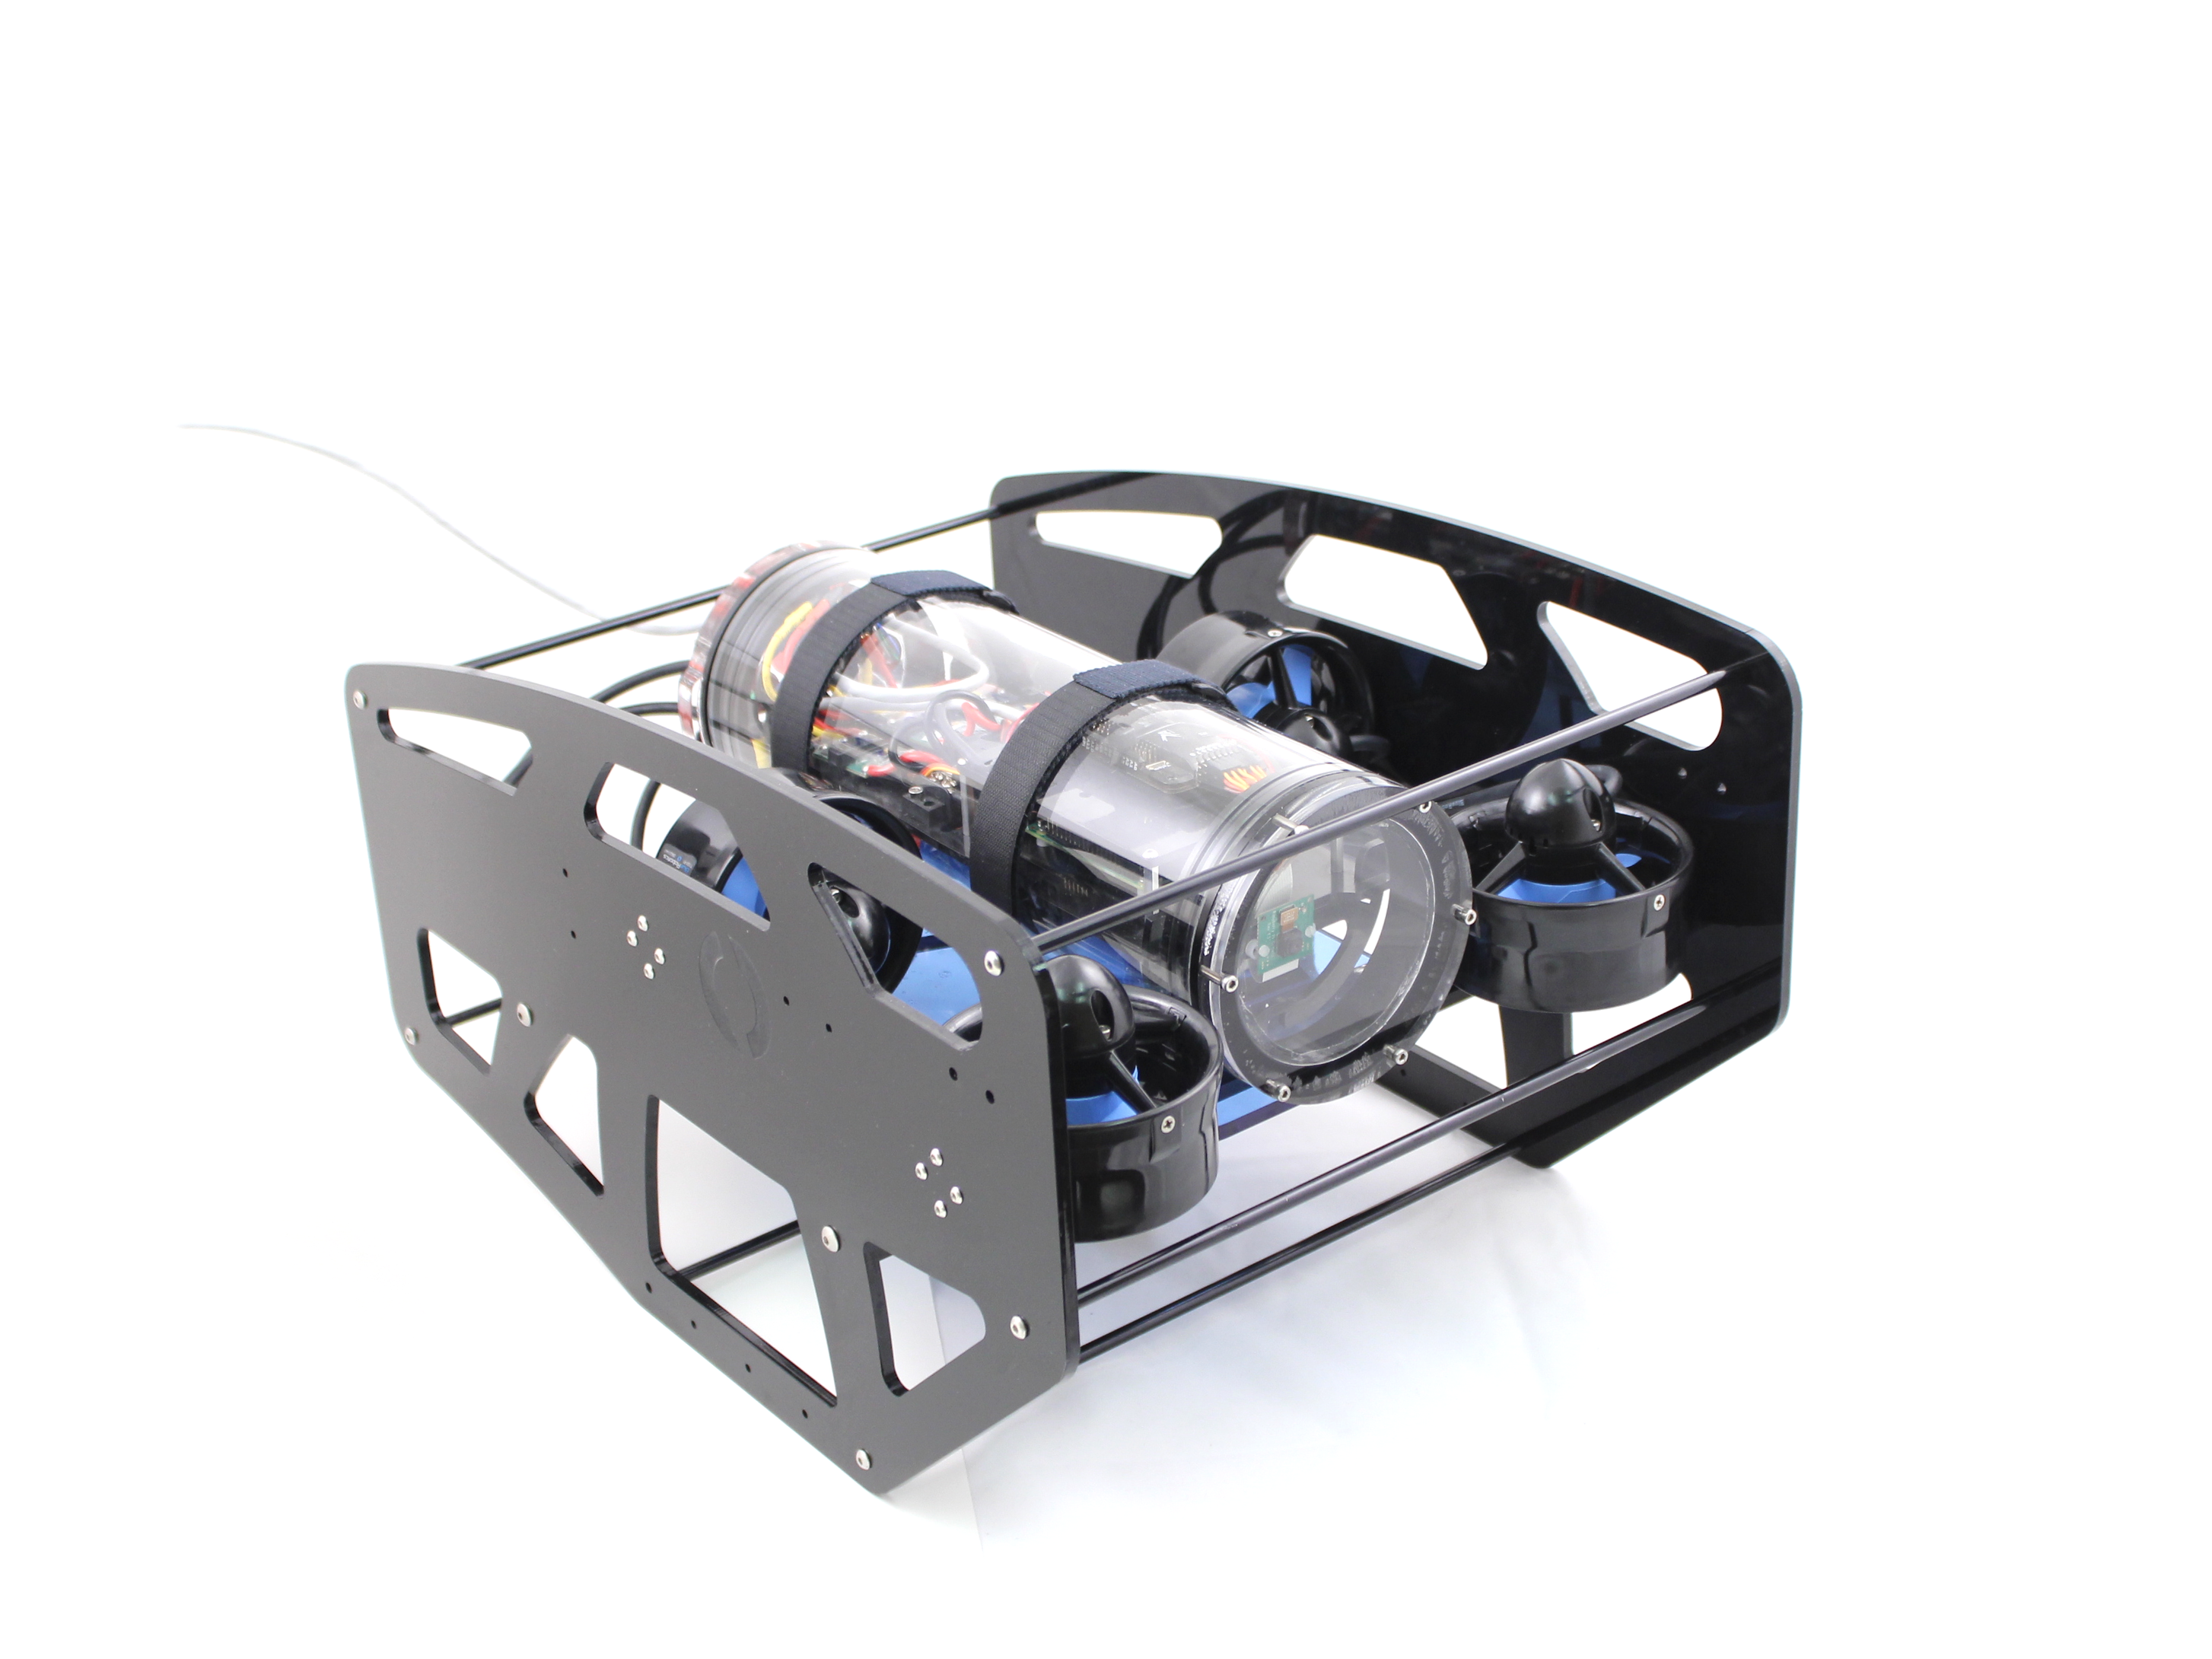
\includegraphics[width = 1.0\textwidth]{Images/Bluerov.png}
		\end{figure}
	\end{block}
	\column[content...]{0.68\textwidth}
	\begin{block}{Model for control design}
		\scriptsize
		\[
		\begin{array}{rl}
		\dot{\mathbf{p}} & =  \mathbf{R} \mathbf{V} \label{eq:kinematicsPos}\\
		\dot{\mathbf{R}} & =  \mathbf{R} \mathbf{\Omega}_\times \\
		\mathbf{M}\dot{\mathbf{V}} &= (\mathbf{M}\mathbf{V}) \!\times\!\mathbf{\Omega} + \mathbf{F}_c + \mathbf{F}_{gb} + \mathbf{F}_d(\mathbf{V}) +\mathbf{\Delta}_F  \\
		\mathbf{J}\dot{\mathbf{\Omega}} &=  (\mathbf{J}\mathbf{\Omega}) \!\times\! \mathbf{\mathbf{\Omega}} + \mathbf{\Gamma}_c + \mathbf{\Gamma}_g +  \mathbf{\Delta}_{\Gamma}
		\end{array} 
		\]
		
		
		\noindent with the ``disturbance'' terms: 
		\[
		\begin{array}{rl}
		\mathbf{\Delta}_F =\!\!\!\!\!\!& -(\mathbf{M}\mathbf{V}_f)_\times \mathbf{\Omega} -\mathbf{M} \mathbf{\Omega}_\times \mathbf{V}_f + (\mathbf{D}^\top \mathbf{\Omega})_\times \mathbf{\Omega} -\mathbf{D}^\top \dot{\mathbf{\Omega}}\\
		&+ \mathbf{F}_d(\mathbf{V}_h) - \mathbf{F}_d(\mathbf{V}) \\
		\mathbf{\Delta}_{\Gamma} =\!\!\!\!\!\! &(\mathbf{DV}_h)\!\times \!\mathbf{\Omega} + \mathbf{P}_h \!\times \!\mathbf{V}_h  - \mathbf{D}\dot{\mathbf{V}}_h  + \mathbf{\Gamma}_d\vspace{-0.1cm}
		\end{array} %\vspace{-0.1cm}
		\]
	\end{block}
\end{columns}
	
\end{frame}


\begin{frame}{Homography}
\begin{columns}
	\column[content...]{0.4\textwidth}
	\begin{block}{Homography}
		\begin{equation*}\label{def:homo}
		\mathbf{H} = \mathbf{R}^{\!\top} - \frac{1}{d^\star} \mathbf{R}^{\!\top} \mathbf{p}_C \mathbf{n}^{\star\!\top} 
		\end{equation*}
	\end{block}
	\column[content...]{0.5\textwidth}
	\begin{block}{Pose decomposition}
		\begin{itemize}
			\item No need!
		\end{itemize}
	\end{block}

	\begin{block}{Visual errors}
		\[
		\begin{array}{rl}
			\mathbf{e}_p &\triangleq (\mathbf{I}_3 - \mathbf{H})\mathbf{m}^\star\\
			\mathbf{e}_\Theta &\triangleq \mathrm{vex}(\mathbf{H}^\top - \mathbf{H}) 
		\end{array}
		\]		
	\end{block}
	\begin{block}{Control objective}
		\[
		\begin{array}{rl}
		(\mathbf{R}, \mathbf{p}_c) & \longrightarrow (\mathbf{I}_3, \mathbf{0})\\
		\mathbf{H} & \longrightarrow \mathbf{I}_3\\
		(\mathbf{e}_p, \mathbf{e}_\Theta) & \longrightarrow (\mathbf{0}, \mathbf{0})
		\end{array}
		\]	
	\end{block}
	
\end{columns}

\end{frame}

\begin{frame}{Kinematic control}
	\begin{block}{S.Benhimane and E.Malis, 2007}
		Homography-based 2D visual tracking and servoing
	\end{block}
	\begin{columns}
		\column[placement]{0.5\textwidth}
		\begin{block}{Lemma 1}
			The kinematic control law
			\begin{equation*}\label{maliscontrol}
			\mathbf{V}_{C} = -k_p \mathbf{e}_p\,,\quad \mathbf{\Omega} = -k_\Theta \mathbf{e}_\Theta  
			\end{equation*}
			with $k_p, k_\Theta>0$, ensures the local exponential stability of $\mathbf{H}  \longrightarrow \mathbf{I}_3$.
		\end{block}
		\column[placement]{0.5\textwidth}
	\end{columns}
\end{frame}




\begin{frame}{Inner-outer loop control architecture}
%Block diagram of the proposed HBVS controller
\begin{figure}
	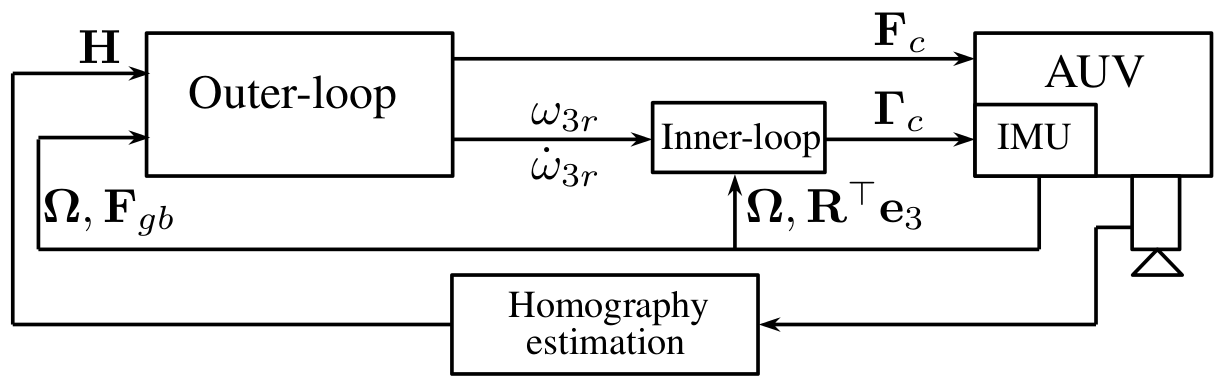
\includegraphics[width = 90mm]{Images/Block_diagram_2.png}
\end{figure}


\begin{itemize}
	\item Inner loop:
	\begin{itemize}
	
		\item $\mathbf{\Gamma}_C$ ensures  $ \mathbf{\Omega} \longrightarrow $ $ \mathbf{\Omega}_r \stackrel{\triangle}{=}  k_g \mathbf{e}_3 \times \mathbf{R}^{T} \mathbf{e}_3 + \omega_{3r} \mathbf{e}_3$ 
	\end{itemize} 
	\item Outer loop:
\end{itemize}
\end{frame}

\begin{frame}{Outer-loop control design}
\begin{itemize}
	\item Without sea currents
	
	\item With sea currents, integral action
\end{itemize}

\end{frame}

\begin{frame}{Inner-loop control design}
\end{frame}

\section{Simulation results}
\begin{frame}{Simulation results}
\end{frame}



\section{Conclusion}

\begin{frame}{Conclusion}

  % Keep the summary *very short*.
  An inertial-aided image-based visual servo controller for the stabilisation of compacted fully actuated AUVs:
  \begin{itemize}
  \item
    %The \alert{first main message} of your talk in one or two lines.
    Using image-based homography without its decomposition.
  \item
    Without relying on linear velocity measurement
  \item
    Locally exponential stability, robustness to unmodeled dynamics and disturbance.
  \end{itemize}
  
  % The following outlook is optional.
  \vskip0pt plus.5fill
  \begin{itemize}
  \item
    A testing campaign is on-going.    
  \end{itemize}
\end{frame}


\begin{frame}
\centering {
	{\huge \textbf{Thank you for your attention!}}	
	{\huge \textbf{Q\&A}}}

\end{frame}



% All of the following is optional and typically not needed. 
%\appendix
%\section<presentation>*{\appendixname}
%\subsection<presentation>*{For Further Reading}
%
%\begin{frame}[allowframebreaks]
%  \frametitle<presentation>{For Further Reading}
%    
%  \begin{thebibliography}{10}
%    
%  \beamertemplatebookbibitems
%  % Start with overview books.
%
%  \bibitem{Author1990}
%    A.~Author.
%    \newblock {\em Handbook of Everything}.
%    \newblock Some Press, 1990.
% 
%    
%  \beamertemplatearticlebibitems
%  % Followed by interesting articles. Keep the list short. 
%
%  \bibitem{Someone2000}
%    S.~Someone.
%    \newblock On this and that.
%    \newblock {\em Journal of This and That}, 2(1):50--100,
%    2000.
%  \end{thebibliography}
%\end{frame}

\end{document}


